\documentclass[a4paper,12pt]{article} 
\usepackage[T2A]{fontenc} %кодировка  
\usepackage[utf8]{inputenc} %Кодировка исходного текста  
\usepackage[english,russian]{babel} %локализация и переносы  
\usepackage[utf8]{inputenc} 
% \usepackage[russian]{babel} 
\usepackage{indentfirst} 
\usepackage{float} 
\usepackage{geometry} 
\usepackage[warn]{mathtext} 
\usepackage[english,russian]{babel} 
\usepackage{amsmath}
\setlength{\parindent}{12.5mm}
% \setlength{\parskip}{1em}
\linespread{1.5} 
\geometry{a4paper,total={170mm,257mm},left=30mm,top=20mm,right=20mm} 
\usepackage{amsmath,amsfonts,amssymb,amsthm,mathtools} %Математика 

\begin{document}
% НАЧАЛО ТИТУЛЬНОГО ЛИСТА
\begin{center}
    \hfill \break
    \large{МИНИСТЕРСТВО НАУКИ И ВЫСШЕГО ОБРАЗОВАНИЯ РОССИЙСКОЙ ФЕДЕРАЦИИ }\\
    \footnotesize{ФЕДЕРАЛЬНОЕ ГОСУДАРСТВЕННОЕ БЮДЖЕТНОЕ ОБРАЗОВАТЕЛЬНОЕ УЧРЕЖДЕНИЕ}\\ 
    \footnotesize{ВЫСШЕГО ПРОФЕССИОНАЛЬНОГО ОБРАЗОВАНИЯ}\\
    \small{\textbf{«МОСКОВСКИЙ АВИАЦИОННЫЙ ИНСТИТУТ»\\(Национальный исследовательский университет)}}\\ \hline
    \hfill \break
    \normalsize{Институт №1}\\
    \normalsize{Кафедра 106}\\
    \hfill\break
    \hfill \break 
    \hfill \break 
    \hfill \break 
\hfill \break 
    \large{\textbf{Лабораторная работа} \\ по дисциплине «Управление движением ЛА» }\\

    \normalsize{«АВТОМАТИЧЕСКАЯ ПОСАДКА САМОЛЕТА ПО ГЛИССАДЕ»}\\
\end{center}
\hfill \break

\normalsize{ 
\begin{flushleft}
\hfill \break 
\hfill \break 
\hfill \break 
\hfill \break 
\hfill \break 
\hfill \break 
\hfill \break 
\hfill \break 
\hfill \break 
    \underline{Выполнили:} \\ \hfill \break 
    А.Е. Пащенко Р.А. Зарубин\\
    «\underline{\hspace{1cm}}» \underline{\hspace{3cm}} 2022 г. \\ \hfill \break
\end{flushleft}
}\\

\begin{center} Москва 2022 \end{center}
\thispagestyle{empty} % выключаем отображение номера для этой страницы!!
 \newpage
% КОНЕЦ ТИТУЛЬНОГО ЛИСТА


\textbf{Цель работы}: исследование системы автоматической посадки самолета по глиссаде с помощью математического моделирования на персональном компьютере. Рассматривается плоская задача продольного движения. Работа содержит:
\begin{itemize}
    \item \textbf{Лабораторная работа №3. Исследования системы автоматической посадки самолета при позиционном регуляторе в контуре глиссады.}
    \item \textbf{Лабораторная работа №4. Исследование системы автоматической посадки самолета при форсирующем регуляторе в контуре глиссады.}
\end{itemize}

\section{Теоретический минимум}

Полет по глиссаде начинается с момента прохождения самолетом  точки 1 на рис.\ref{fig:Полёт по глисаде} С этого момента начинается снижение самолета по сигналам глиссадного маяка до высоты порядка 20 м, пока имеется устойчивый сигнал глиссадного радиомаяка (ГРМ). Стабилизация самолета относительно глиссады в этом случае производится путем изменения угла тангажа самолета. Это обеспечивается каналом руля высоты.

\begin{figure}[H]
    \center{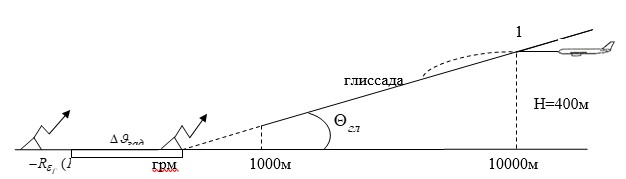
\includegraphics[width=\linewidth]{figures/1.jpg}}
    \caption{Полёт по глисаде}
    \label{fig:Полёт по глисаде}
\end{figure}

При полете по глиссаде самолет должен снижаться с постоянной скоростью. Выполнение этого требования возлагается на автомат тяги, который стабилизирует заданное значение скорости.

Схема аппаратурного построения канала руля высоты системы автоматической посадки по глиссаде приведена на рис. \ref{fig:Cистема автоматической посадки по глиссаде}

\begin{figure}[H]
    \center{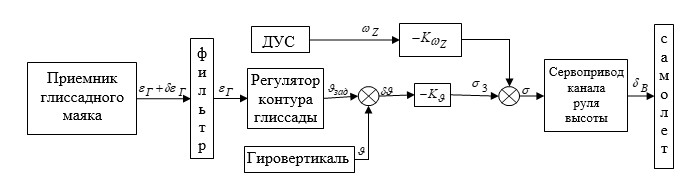
\includegraphics[width=\linewidth]{figures/2.jpg}}
    \caption{Cистема автоматической посадки по глиссаде}
    \label{fig:Cистема автоматической посадки по глиссаде}
\end{figure}

Для формирования контура управления продольным движением при полете самолета по глиссаде рассмотрим геометрию движения по радиолучу (рис. \ref{fig:Полёт по глисаде 2}). Из рис. \ref{fig:Полёт по глисаде 2} видно, что $\varepsilon_\text{Г} = \frac{d}{D} $ и $\dot{d} = V\Delta \theta$. Отсюда находим связь между $\varepsilon_\text{Г}$ и $\Delta \theta$. Проводя преобразования Лапласа, при замороженном значении дальности $D$ получаем:

$$ \varepsilon_\text{Г} = \frac{V}{D} \cdot \frac{1}{p} \cdot \Delta \theta  $$

\begin{figure}[H]
    \center{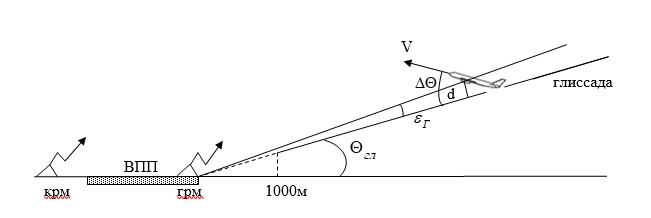
\includegraphics[width=\linewidth]{figures/3.jpg}}
    \caption{Полёт по глисаде}
    \label{fig:Полёт по глисаде 2}
\end{figure}

С учетом полученного соотношения структурная схема контура управления движением самолета по глиссаде в пренебрежении динамикой измерителей и сервопривода принимает вид, приведенный на рис. \ref{fig:Cистема автоматической посадки по глиссаде 2}. Введение внутренних контуров по угловой скорости $\omega_z$ и углу тангажа $\vartheta$  позволяет улучшить характеристики устойчивости и управляемости самолета, т.е. улучшить динамические характеристики самолета и расширить область возможных частот управления.

\section{Модель исследуемой системы}
\label{eq: СДУ}
\begin{equation}
    \begin{cases}
    \dot{\omega_z} = K_{z}m_z^{\bar{\omega}_z}\frac{b_a}{V} \omega_z + K_z m_z^{\alpha} \alpha + K_z m_z^{\dot{\alpha}} \frac{b_a}{V} \dot{\alpha} + K_z m_z^{\delta_\text{в}}\\
    \dot{\alpha} = \omega_z - \bar{Y}^\alpha \alpha \\ 
    \dot{\vartheta} = \omega_z \\ 
    \dot{V_y} = V \cdot \bar{Y}^\alpha
\end{cases}
\end{equation}

При исследовании автоматической посадки самолета эту систему необходимо дополнить кинематическим уравнением для угла $\varepsilon_{\text{Г}}$:
$$\dot{\varepsilon_\text{Г}}=\frac{V}{D} \theta$$
и угла наклона траектории:
$$\theta = \vartheta - \alpha$$.

Кроме того, вводятся уравнения автопилота, выражающие закон управления рулем высоты:

\begin{equation}
    \delta_B = K_{\omega_z} \omega_z - K_{\vartheta}(\vartheta_{\text{зад}}-\vartheta) \\ 
\end{equation}
$$\delta_\text{зад} = -(K_{\varepsilon_\text{Г}}\varepsilon_\text{Г}+K_{\dot{\varepsilon}_\text{Г}}\dot{\varepsilon}_\text{Г})$$




\end{document}
